% This file was created with tikzplotlib v0.10.1.
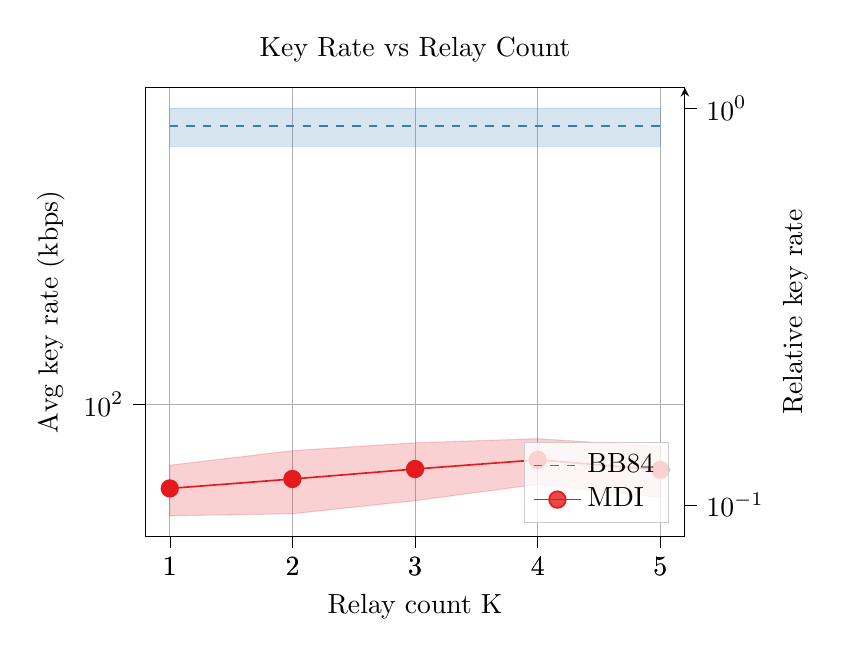
\begin{tikzpicture}

\definecolor{crimson2282628}{RGB}{228,26,28}
\definecolor{darkgray176}{RGB}{176,176,176}
\definecolor{darkorange25512714}{RGB}{255,127,14}
\definecolor{lightgray204}{RGB}{204,204,204}
\definecolor{steelblue31119180}{RGB}{31,119,180}
\definecolor{steelblue55126184}{RGB}{55,126,184}

\begin{axis}[
legend cell align={left},
legend style={
  fill opacity=0.8,
  draw opacity=1,
  text opacity=1,
  at={(0.97,0.03)},
  anchor=south east,
  draw=lightgray204
},
log basis y={10},
tick align=outside,
tick pos=left,
x grid style={darkgray176},
xlabel={Relay count K},
xmajorgrids,
xmin=0.8, xmax=5.2,
xtick style={color=black},
xtick={1,2,3,4,5},
xticklabels={
  \(\displaystyle {1}\),
  \(\displaystyle {2}\),
  \(\displaystyle {3}\),
  \(\displaystyle {4}\),
  \(\displaystyle {5}\)
},
y grid style={darkgray176},
ylabel={Avg key rate (kbps)},
ymajorgrids,
ymin=42.213776033326, ymax=788.725804098587,
ymode=log,
ytick style={color=black},
ytick={1,10,100,1000,10000},
yticklabels={
  \(\displaystyle {10^{0}}\),
  \(\displaystyle {10^{1}}\),
  \(\displaystyle {10^{2}}\),
  \(\displaystyle {10^{3}}\),
  \(\displaystyle {10^{4}}\)
}
]
\path [draw=steelblue55126184, fill=steelblue55126184, opacity=0.2]
(axis cs:1,690.449428720482)
--(axis cs:1,538.07315917704)
--(axis cs:2,538.07315917704)
--(axis cs:3,538.07315917704)
--(axis cs:4,538.07315917704)
--(axis cs:5,538.07315917704)
--(axis cs:5,690.449428720482)
--(axis cs:5,690.449428720482)
--(axis cs:4,690.449428720482)
--(axis cs:3,690.449428720482)
--(axis cs:2,690.449428720482)
--(axis cs:1,690.449428720482)
--cycle;

\path [draw=crimson2282628, fill=crimson2282628, opacity=0.2]
(axis cs:1,67.1050158242511)
--(axis cs:1,48.2223506327235)
--(axis cs:2,48.8846985020699)
--(axis cs:3,53.2285501437557)
--(axis cs:4,59.2179181130866)
--(axis cs:5,54.3758080129703)
--(axis cs:5,75.7943815265278)
--(axis cs:5,75.7943815265278)
--(axis cs:4,79.783221055613)
--(axis cs:3,77.6827748193142)
--(axis cs:2,73.7805572065294)
--(axis cs:1,67.1050158242511)
--cycle;

\addplot [semithick, steelblue55126184, dashed]
table {%
1 614.261293948761
2 614.261293948761
3 614.261293948761
4 614.261293948761
5 614.261293948761
};
\addlegendentry{BB84}
\addplot [semithick, crimson2282628, mark=*, mark size=3, mark options={solid}]
table {%
1 57.6636832284873
2 61.3326278542996
3 65.4556624815349
4 69.5005695843498
5 65.085094769749
};
\addlegendentry{MDI}
\end{axis}

\begin{axis}[
axis y line=right,
log basis y={10},
tick align=outside,
title={Key Rate vs Relay Count},
x grid style={darkgray176},
xmin=0.8, xmax=5.2,
xtick pos=left,
xtick style={color=black},
y grid style={darkgray176},
ylabel={Relative key rate},
ymin=0.0834020432354434, ymax=1.12557007592045,
ymode=log,
ytick pos=right,
ytick style={color=black},
ytick={0.001,0.01,0.1,1,10,100},
yticklabel style={anchor=west},
yticklabels={
  \(\displaystyle {10^{-3}}\),
  \(\displaystyle {10^{-2}}\),
  \(\displaystyle {10^{-1}}\),
  \(\displaystyle {10^{0}}\),
  \(\displaystyle {10^{1}}\),
  \(\displaystyle {10^{2}}\)
}
]
\addplot [semithick, steelblue31119180, opacity=0]
table {%
1 1
2 1
3 1
4 1
5 1
};
\addplot [semithick, darkorange25512714, opacity=0]
table {%
1 0.0938748441364391
2 0.0998477821384847
3 0.106559965809916
4 0.113144960082976
5 0.105956692063977
};
\end{axis}

\end{tikzpicture}
